\chapter{DeSTIN算法的介绍与测试}\label{chapter_algorithm}
\graphicspath{{chapter3/figure/}}

本章我们将对我们研究的深度空时关系推断网络(Deep SpatioTemporal Inference Network,DeSTIN)进行介绍;并且基于此进行测试,分析其算法的可靠性以及移植到硬件上的可能性。

\section{DeSTIN算法介绍}

上一章笔者介绍了一些常见的深度学习方法。这些方法在应对“维度困境”,在高维度数据处理和特征提取上产生了不错的成果。但是这些算法应用的方面有一定的局限性:这些方法都以处理静态问题为主,不能很好地处理包含时间序列的问题。虽然在深度神经网络(DNN)的基础上发展出了一种循环神经网络(Recurrent Neural Network,RNN)的方法,但是其具有DNN方法与生俱来的缺陷:全连接网络,计算效率较差;很深的反向传播距离使得其训练较为困难。

我们将首先从概率论的角度进行时间序列问题解决方案的描述,再进一步落实到我们使用的DeSTIN算法上来。随后我们将对DeSTIN算法做一些数据集测试,检验其学习能力以及缺陷。

\subsection{DeSTIN算法的理论基础}

本节的理论分析主要基于DeSTIN的第一篇论文。\cite{Arel2009DeSTIN}

我们考虑\uline{在一个深层神经网络结构里,为了准确反映时间序列关系,一个神经节点应当如何进行其信度状态更新}的问题。

我们首先做一个假设:\uline{被观测的数据的序列结构能够被结构化地表示出来;于此同时,序列里两件事的长程相关性不会和这两件事的间隔准确地相关}。

这个假设让我们对数据的结构有一个先验的判断:其结构能够被多层的网络状态抽象提取出来。于此同时,由于数据的长程相关性不与间隔严格相关,我们可以采用一个相对粗糙时序度量。

我们主要讨论\uline{一个神经网络节点下一时刻的信度状态如何由当前自身的信度状态、母节点的信度状态和当前的观测值来确定}。整个神经网络接收一个外界输入的序列集,并尝试从序列集中提取特征规律,通过自身的信度状态表达出来。

现对后续讨论的符号进行规定:假设我们讨论的节点在当前时刻的信度状态为$b(s)$,其中s指\uline{输入节点的任何可能的状态序列},S指整个状态序列的空间(序列集);此节点存在母节点,其信度状态为$c$;此节点下一个时刻的信度状态为$b^\prime(s^\prime)$;当前观测值记为$o$。

由信度状态的定义以及以上假设知:
\begin{equation}
b^\prime(s^\prime) = Pr(s^\prime|o,b,c) = \dfrac{Pr(s^\prime, o, b, c)}{Pr(o, b, c)}
\end{equation}

由条件概率公式,上式可以化为:
\begin{equation}
b^\prime(s^\prime) = \dfrac{Pr(o|s^\prime,b,c)Pr(s^\prime|b,c)Pr(b,c)}{Pr(o|b,c)Pr(b,c)}
\end{equation}

我们再假设:\uline{观测值不依赖于节点的信度状态b、c,只依赖于输入的序列状态$s$、$s^\prime$},那么$Pr(o|s^\prime,b,c) = Pr(o|s^\prime)$,上式进一步简化为:

\begin{equation}
b^\prime(s^\prime) = \dfrac{Pr(o|s^\prime)Pr(s^\prime|b,c)}{Pr(o|b,c)}
\end{equation}

此处$Pr(s^\prime|b,c) = \sum_{s\in S} Pr(s^\prime|s,c) b(s)$,进一步改写上式:

\begin{equation}
\label{eqn:destin}
b^\prime(s^\prime) = \dfrac{Pr(o|s^\prime)\sum_{s\in S} Pr(s^\prime|s,c) b(s)}{\sum_{s^{\prime\prime}\in S}Pr(o|s^{\prime\prime})\sum_{s\in S} Pr(s^{\prime\prime}|s,c) b(s)}
\end{equation}

此时分母为归一化因子。我们考虑公式\ref{eqn:destin}中分子每一项的意义。$Pr(o|s^\prime)$反映出模式静态的相似度(当前的观测值与之后输入序列的关系);而$Pr(s^\prime|s,c)$\uline{反映系统演化过程}(当前输入序列,母节点信度与之后输入序列的关系)。在我们的结构中,母节点的信度状态$c$通过以下方式进行选择:

\begin{equation}
c = arg\;max_s b_p(s)
\end{equation}

其中$b_p(s)$为母节点的信度关于输入状态的分布。即我们取使母节点信度最大的输入状态$s$作为$c$。

我们重新考察式\ref{eqn:destin},可知:如果我们能够较好地获得$Pr(o|s^\prime)$和$Pr(s^\prime|s,c)$的表示,就可以由当前信度状态和观测推知下一个时刻的信度状态,即进行了序列特征的识别。

文章\cite{Arel2009DeSTIN}中基于式\ref{eqn:destin}进行了说明:$Pr(o|s^\prime)$可以通过\uline{在线聚类方法}进行学习(见第二章k-means聚类小节);而$Pr(s^\prime|s,c)$由神经网络的结构关联进行反映。

基于以上理论,我们展开DeSTIN算法的介绍。

\subsection{DeSTIN算法的整体框架}

DeSTIN构架的网络结构如图\ref{fig:destinarchi}。其借鉴了深度信念网络的想法:在层与层之间传递节点学习的信度状态(Belief State),将下面一层的四个(或者两个)相邻的子节点信度的状态合并,作为上面一层节点的输入信号。

对于每一个节点,信度状态具体体现为:节点内部进行聚类计算,判断输入的数据$o$输入分别属于其内部k个聚类的概率:${P(h_i|o)}_{i:1\sim k}$,将这一组概率称为其输出的信度状态。

\begin{figure}[htbp]
   \centering
   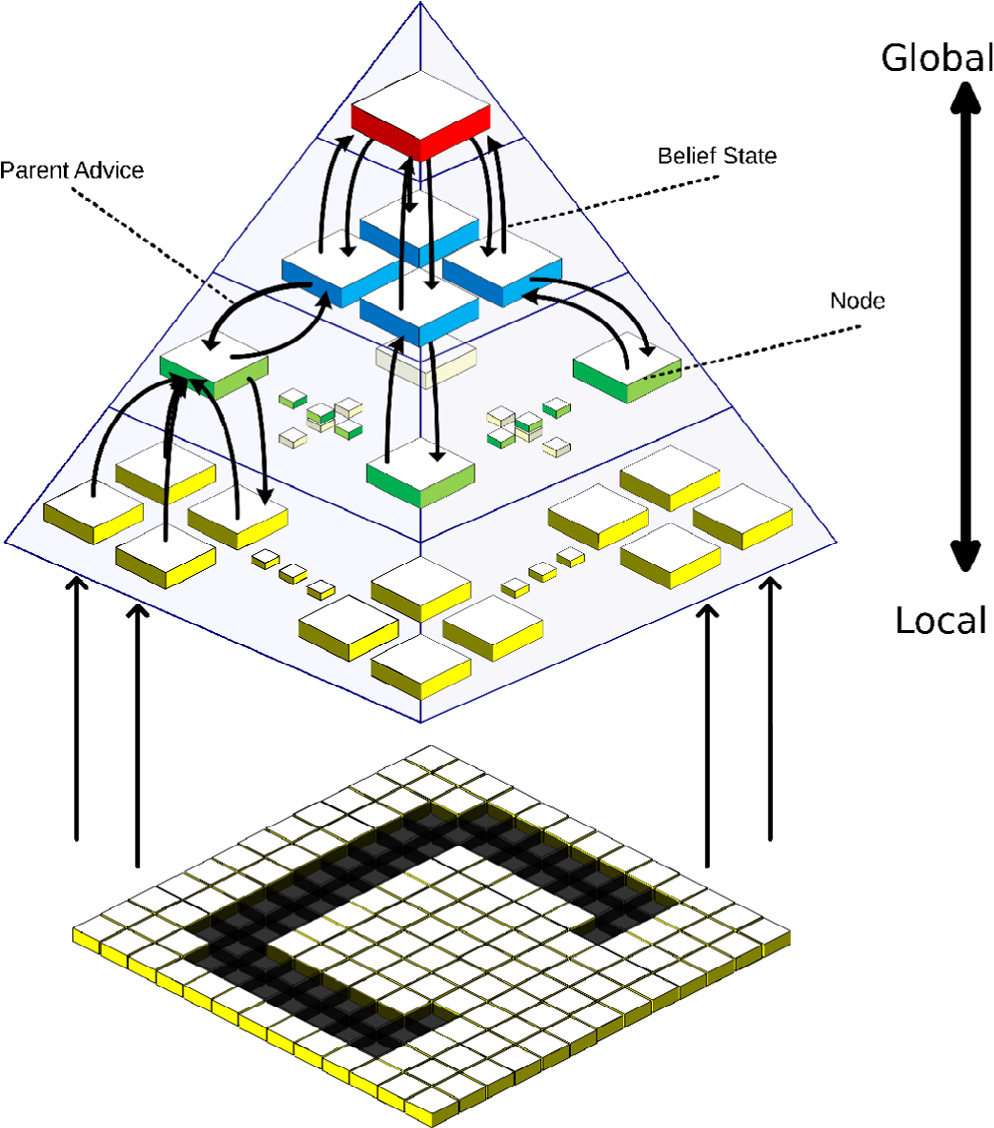
\includegraphics[width=0.5\textwidth]{DeSTINArchitecture.png} % requires the graphicx package
   \caption{DeSTIN算法的架构}
   \label{fig:destinarchi}
\end{figure}

对于整个结构,数据序列由底层逐个输入,底层神经元根据输入数据调整自身的参数,尝试获得其中较为显著的空间、时间关系,将其体现在信度状态的输出中;上一层接收到下一层的信度状态输入后,尝试捕捉\uline{更加宏观的空间时间关系},并进行自身权重调整;整个结构由下往上来看,\uline{提取的空间时间特征不断地全局化,最终每一层都产生不同层次的特征提供给后续的监督学习}。

\subsection{单个神经元的online k-means聚类算法}
以下我们详细介绍单个神经元采用的online k-means clustering算法,分析其如何进行学习、以及输出信度状态的。

根据整体DeSTIN结构的要求,一个具体的神经元应当具有如图\ref{fig:neuronstr}的结构。

\begin{figure}[htbp]
   \centering
   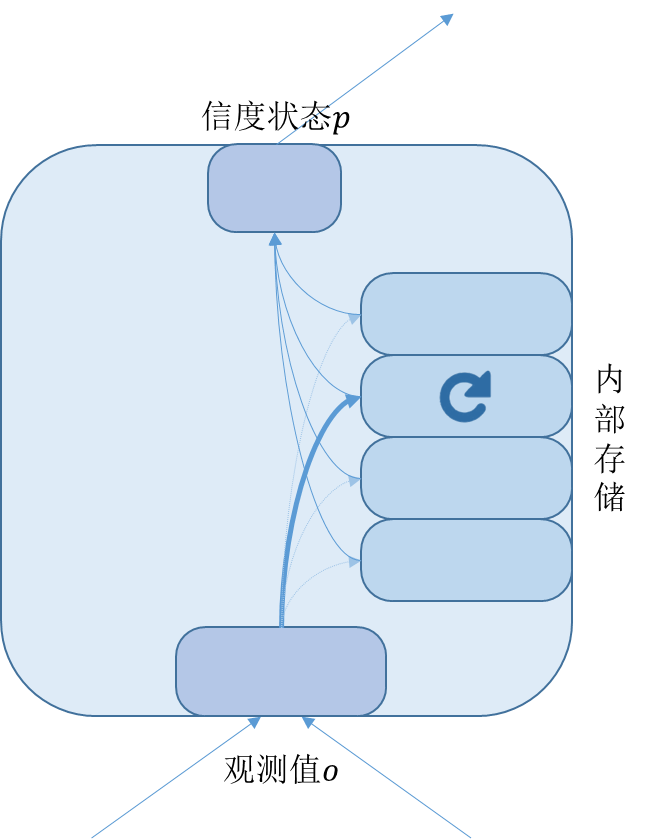
\includegraphics[width=0.4\textwidth]{NeuronStructure.png} % requires the graphicx package
   \caption{DeSTIN神经元的抽象结构}
   \label{fig:neuronstr}
\end{figure}

每一个任务周期内,神经元将按顺序执行以下步骤:
\begin{enumerate}
\item 聚类判断过程: 接收输入信号$o$(底层为数据输入,上层为下层的信度状态输入);根据自己的聚类参数判断其属于哪一个聚类;
\item 学习过程: 根据输入数据更新自身的聚类特性;
\item 信度计算过程: 根据$o$以及更新后的聚类参数计算其属于每一个聚类的概率,作为信度状态输出。
\end{enumerate}

我们将以上过程具体化。假设输入的观测值为$o$,为了可视化方便起见,假设输入数据$o$为I=2维;按照传统聚类的方法,我们初始化J个聚类(此处$J=4$),其中心为$\{\mu_j\}$,参数方差为(高斯分布)$\{\sigma^2_j\}$,注意到$\mu_j, \sigma^2_j$均为I维的向量。如图\ref{fig:onlineclus1}所示。

\begin{figure}[htbp]
   \centering
   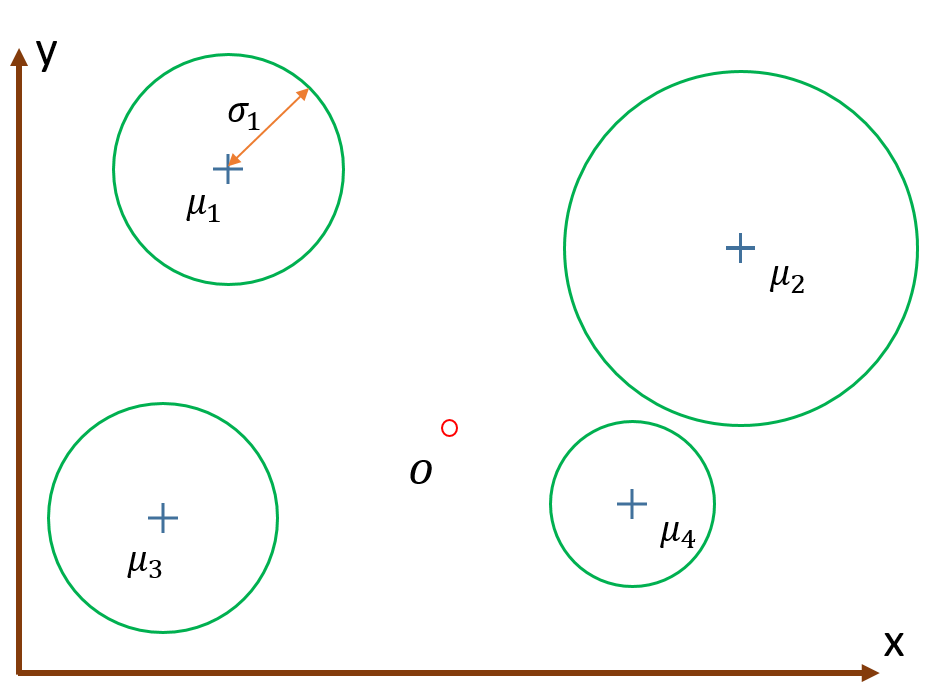
\includegraphics[width=0.5\textwidth]{OnlineClustering1.png} % requires the graphicx package
   \caption{聚类算法1:参数以及初始化}
   \label{fig:onlineclus1}
\end{figure}

首先,我们执行聚类判断过程:如图\ref{fig:onlineclus2},我们采取“赢家通吃(Winner-Takes-All)”的原则进行聚类的判断:根据欧氏距离(的平方)$d_j = ||o - \mu_j||^2$来判断聚类归属,最小者胜利,具体公式如下:
\begin{equation}
j0 = arg\;min_j d_j = arg\;min_j ||o - \mu_j||^2
\end{equation}

\begin{figure}[htbp]
   \centering
   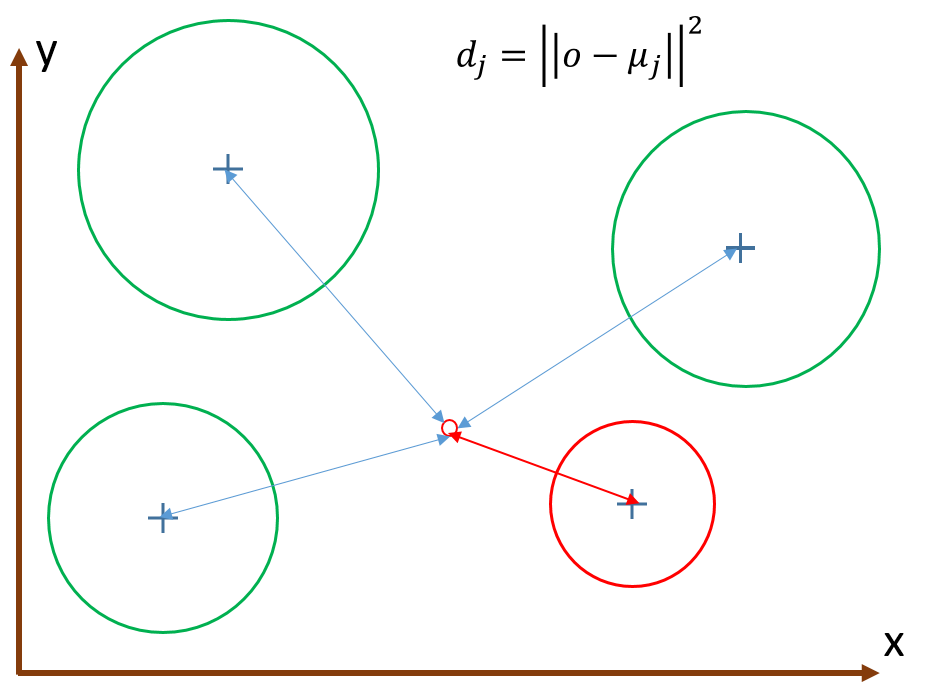
\includegraphics[width=0.5\textwidth]{OnlineClustering2.png} % requires the graphicx package
   \caption{聚类算法2:聚类判断过程}
   \label{fig:onlineclus2}
\end{figure}

然后,我们进行赢家的聚类更新:如图\ref{fig:onlineclus3},设定圆心聚类学习速率为$\alpha$,方差聚类学习速率为$\beta$,那么:
\begin{equation}
\left\{
\begin{aligned}
\mu_{j0} & \Leftarrow \mu_{j0} + \alpha (o - \mu_{j0}) \\
\sigma^2_{j0} & \Leftarrow \sigma^2_{j0} + \beta (d_{j0} - \sigma^2)  = \sigma^2_{j0} + \beta ((o-\mu_{j0})^2 - \sigma^2)
\end{aligned}
\right.
\end{equation}

\begin{figure}[htbp]
   \centering
   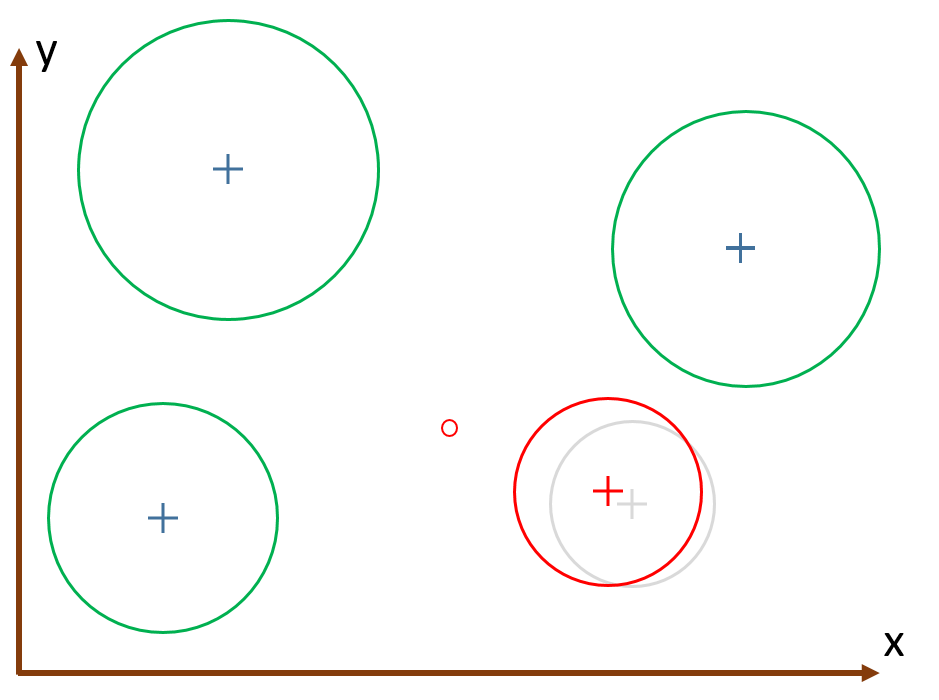
\includegraphics[width=0.5\textwidth]{OnlineClustering3.png} % requires the graphicx package
   \caption{聚类算法3:聚类学习过程}
   \label{fig:onlineclus3}
\end{figure}

最后,我们根据更新后的聚类信息进行信度状态的计算。我们借鉴了Gaussian混合模型里面概率计算的方法,但是进行了简化\cite{Young2014Hierarchical}。如图\ref{fig:onlineclus4},我们根据归一化的Euclid距离$n_j$进行概率估计:当数据点$o$与我们的聚类距离较小时,其属于聚类的概率便较大;我们假设数据的距离与其属于该聚类的概率成反比,那么有:
\begin{equation}
\begin{aligned}
n_j & = \sum_i \dfrac{||o_i-\mu_{i,j}||^2}{\sigma^2_{i,j}} \\
p_j & = \dfrac{n_j^{-1}}{\sum_{j^\prime} n_{j^\prime}^{-1}}
\end{aligned}
\end{equation}

\begin{figure}[htbp]
   \centering
   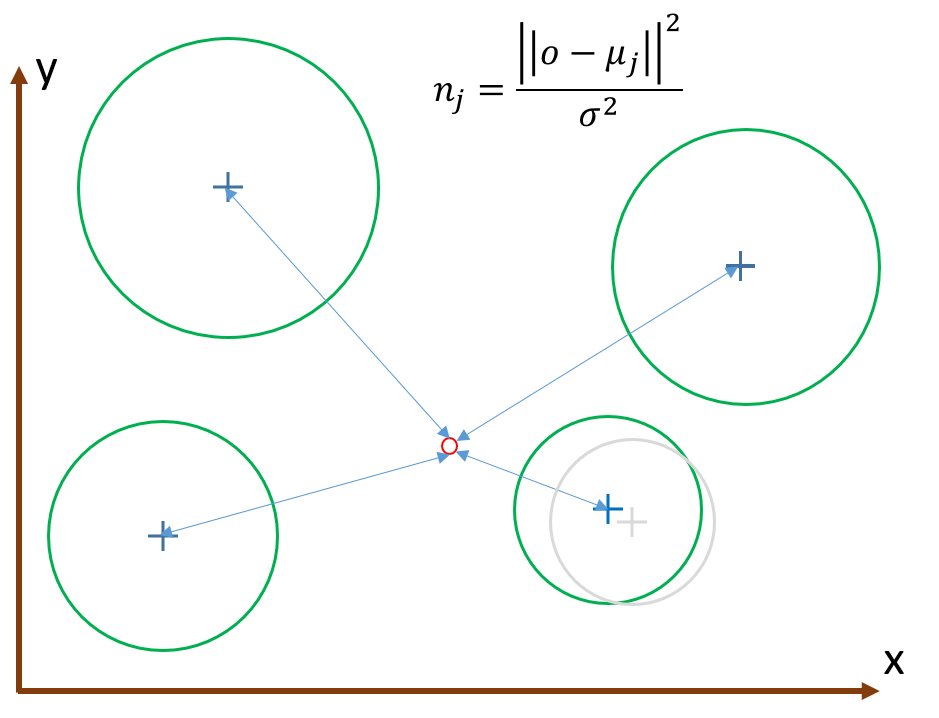
\includegraphics[width=0.5\textwidth]{OnlineClustering4.png} % requires the graphicx package
   \caption{聚类算法4:信度状态计算过程}
   \label{fig:onlineclus4}
\end{figure}

可以看出,我们的算法在传统聚类和混合聚类方法中取了一个平衡:\uline{只更新最近的一个聚类;但是考虑数据点聚类归属时,输出其属于每个聚类的概率},这样既保证计算不会过大,又能够较为准确地反映结果。

我们采用的聚类方法的主要过程介绍完了,但是为了弥补原算法的一个不足之处,我们引入\textbf{饥饿值}的概念\cite{Young2010A}。

我们可以想象一种情况:假设真实的数据有四个团簇,我们也初始化了四个聚类;但是很不幸的是,有一个聚类的初始化距离4个数据团簇都很远;那么每一次更新时该聚类都不能移动,最终这个聚类位置完全不能反映数据团簇情况,称为“\textbf{空闲类}”,而空闲类较多时,聚类数目就不足以反映真实团簇的数目:3个聚类在对应4个数据团簇时效果就没有那么理想了。

为了解决这个问题,我们为每一个聚类再增加一个“饥饿值”参数$\{\psi_j\} (\psi_j:0\sim 1)$:假设在某一个操作周期中,该聚类未被更新,其饥饿程度增大,$\psi$减小;反之$\psi$增大。
\begin{equation}
\psi_j \Leftarrow \left\{
\begin{aligned}
& \gamma \psi_j  \\
& \gamma \psi_j + (1-\gamma)
\end{aligned}
\right.
\end{equation}

其中$\gamma:0\sim1$为“饥饿参数”。这样我们可以保证$\{\psi_j\}$一直处于$0\sim 1$的范围内。如图\ref{fig:onlineclus5},在聚类判断过程中,我们将“饥饿值”也作为考虑的因素,即
\begin{equation}
j0 = arg\;min_j (\psi d_j) = arg\;min_j (\psi ||o - \mu_j||^2 )
\end{equation}

\begin{figure}[htbp]
   \centering
   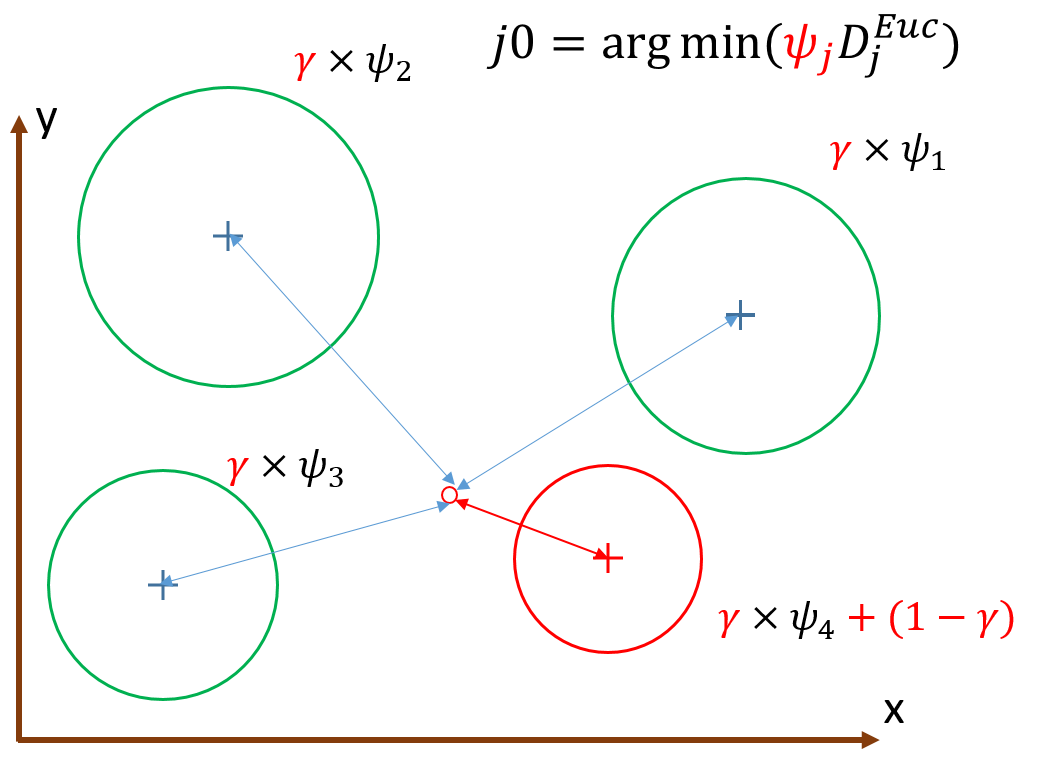
\includegraphics[width=0.5\textwidth]{OnlineClustering5.png} % requires the graphicx package
   \caption{聚类算法5:饥饿值的引入}
   \label{fig:onlineclus5}
\end{figure}

我们将在线聚类算法的过程总结为MATLAB代码如下:

\begin{spacing}{1}
\begin{lstlisting}[language=Matlab][deletekeywords={input, beta, gamma}]
function [belief, mu, sigma2, starve] = OnlineClustering(input, mu, sigma2,starve, alpha, beta, gamma, training)
%% Use Online k-means Clustering method to calculate the belief
% Written by Pei Zeng, PHY, NJU

% Data input to this function: 
% input: input data to the neuron. I-by-1 vector 
% (I is the input dimension,which is defined in DeSTIN.m)
% mu: centroid attribute for the coordinate of center. I-by-J vector
% (J is the belief dimension, which is defined in DeSTIN.m)
% sigma2: centroid attribute for the radius square. I-by-J vector

% New data output from this function:
% belief: new belief state of the neuron: J-by-1 vector

% initialization
I = size(input,1);
J = size(mu, 2);

%% Data Processing
% 1. Calculating the Euclidean distance from the input to each centroid
D_Euc = zeros(J, 1);
for j = 1 : J
    D_Euc(j) = (input - mu(:,j))' * (input - mu(:,j));
end

% 2. Judge which cluster the input belongs to: Winner-take-all method
[~, j0] = min(starve .* D_Euc);

if (training == 1) % do the renewing only in the training process
% 3. Renew the starvation trace of each centroid
starve = starve * gamma;
starve(j0) = starve(j0) + (1 - gamma);

% 4. Calculate the error for the centroid j0 and the input signal
Er_mu = input - mu(:,j0);
Er_sigma2 = (input - mu(:,j0)).* (input - mu(:,j0)) - sigma2(:,j0);

% 5. Learning Process: learning rate : alpha, beta
mu(:,j0) = mu(:,j0) + alpha * Er_mu;
sigma2(:,j0) = sigma2(:,j0) + beta * Er_sigma2;
end

% 6. Calculate the Mahanalobis distance:
D_Mah = zeros(J, 1);
for j = 1 : J
    D_Mah(j) = sum( (input - mu(:,j)).*(input - mu(:,j))./(sigma2(:,j)) );
end

% 7. "Inverse-normalize" the D_Mah values, and attain the new belief state
Sum = sum(1./D_Mah);
belief = (1./D_Mah)/Sum;

\end{lstlisting}
\end{spacing}


\section{DeSTIN算法测试}
我们首先对于DeSTIN算法进行了单个神经元的聚类测试,获得了一些有关于DeSTIN聚类的性质;在此基础上,我们进行了手写数字识别(MNIST)的测试以及彩色物体识别(CIFAR)的测试,进一步分析其优势与缺陷。

\subsection{单个神经元的聚类测试}
我们首先研究一个神经元是否可以较好地完成聚类测试,即当数据逐一输入的时候,聚类算法是否能够有效地找到数据的中心位置。

我们先声明默认的测试环境,见表\ref{tab:clusterpara}。
\begin{table}[htbp]
\centering
\begin{tabular}{c|c}
  \hline
  参数   & 特征 \\
  \hline
  数据空间维数$I$  &   2 \\
  \hline
  样品真实团簇数目$J_{real}$    & 4 \\
  每个团簇的样本数$n$    & 300 \\
  团簇中心$\mu_{real}$    & $\{(0.2,0.2), (0.2,0.6), (0.6,0.2), (0.6,0.6)\}$ \\
  团簇方差$\sigma_{real}$   & $\{(0.1,0.15), (0.1,0.1), (0.15,0.1), (0.05, 0.2)\}$ \\
  \hline
  聚类数目$J$    &  4 \\
  聚类初始化中心$\mu$  &   $0.15 + 0.5*rand(I,J)  \;\; (0.15\sim 0.65)$ \\
  聚类初始方差$\sigma$  &   $ones(I,J)$ \\
  聚类初始饥饿值$\psi$  &    $ones(1,J)$ \\
  \hline
  学习速率$\alpha$  &   0.12 \\
  学习速率$\beta$  &   0.12 \\
  饥饿速率$\gamma$  &   0.98 \\
  \hline
\end{tabular}
\caption{聚类测试的默认参数}
\label{tab:clusterpara}
\end{table}

我们将数据团簇位置选择在$0.2,0.6$的原因是:\uline{为了保证和今后的测试环境类似,使得学习速率、初始化选择具有借鉴性}。由于之后测试集的数据将会被归一化,其数据范围和我们聚类测试接近,这样我们就可以借鉴一些参数测试的经验。

\subsubsection{理想状况}
我们先假设数据集非常理想,样本团簇的方差很小(我们将方差$\sigma_{real}$全部调整为0.05),团簇之间互不交叠,测试的结果如图\ref{fig:clustest1re}。

\begin{figure}[htbp]
   \centering
   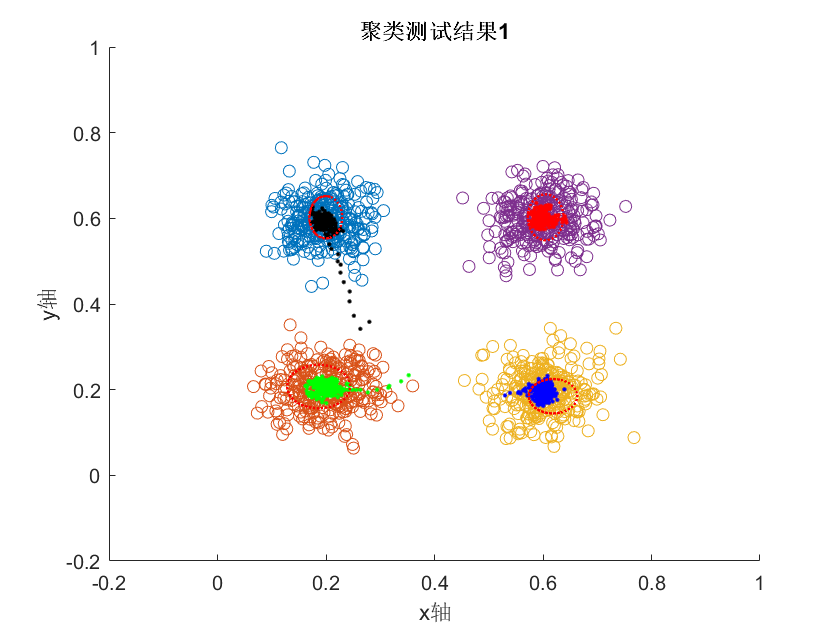
\includegraphics[width=0.7\textwidth]{ClusterTest1Result.png} % requires the graphicx package
   \caption{聚类测试1:理想状况,结果图}
   \label{fig:clustest1re}
\end{figure}

可见聚类效果比较理想。图\ref{fig:clustest1re}中红色椭圆展示了方差的情况,椭圆的圆心位置即为最终聚类的中心位置。而小圆点反映出每一个聚类随着样本逐一输入的的迁移情况。

我们对比最终聚类得到的参数结果和团簇真实值如下:
\begin{table}[htbp]
\centering
\begin{tabular}{c|c||c|c}
  \hline
  $\mu_{real}$   &  $\sigma_{real}$ &  $\mu$  &   $\sigma$\\
  \hline
  $(0.2,0.2)$    &  $(0.05,0.05)$   &  $(0.1864, 0.2073)$  & $(0.0580, 0.0508)$ \\
  $(0.2,0.6)$    &  $(0.05,0.05)$   &  $(0.1997, 0.6025)$  & $(0.0302, 0.0494)$ \\
  $(0.6,0.2)$    &  $(0.05,0.05)$   &  $(0.6185, 0.1847)$  & $(0.0446, 0.0401)$ \\
  $(0.6,0.6)$    &  $(0.05,0.05)$   &  $(0.6048, 0.6025)$  & $(0.0328, 0.0536)$ \\
  \hline
\end{tabular}
\caption{聚类测试1:聚类结果比较}
\label{tab:clustest1}
\end{table}

\subsubsection{常规测试}
接下来,我们采用默认参数进行训练;此时团簇之间存在交叠,并且方差不均一,在两个温度上不对称(见表\ref{tab:clusterpara})。之后的测试团簇的参数不再改变,我们将样本情况画出(符合之后所有的测试样本的情况)。

\begin{figure}[htbp]
   \centering
   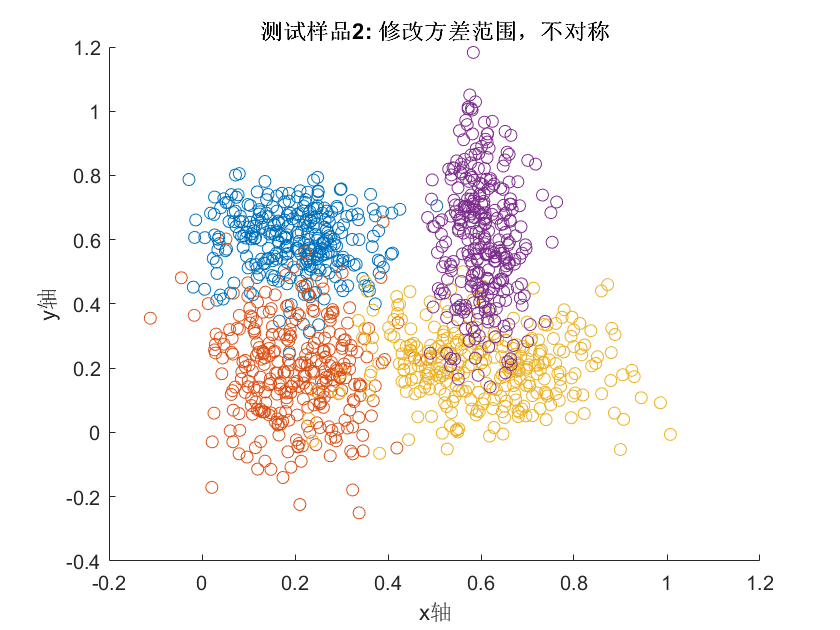
\includegraphics[width=0.7\textwidth]{ClusterTest2Sample.png} % requires the graphicx package
   \caption{聚类测试2:常规测试,样本图}
   \label{fig:clustest2sa}
\end{figure}

测试的结果如图\ref{fig:clustest2re}。

\begin{figure}[htbp]
   \centering
   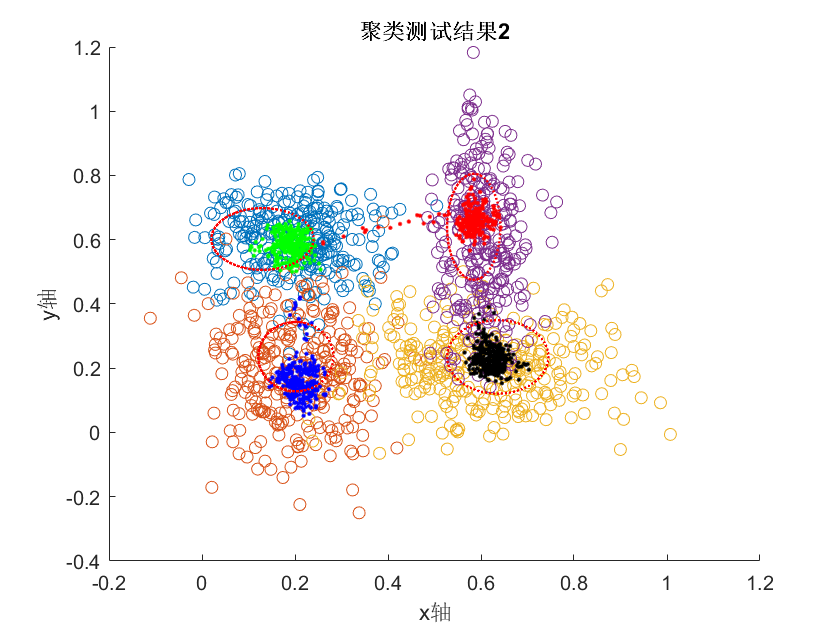
\includegraphics[width=0.7\textwidth]{ClusterTest2Result.png} % requires the graphicx package
   \caption{聚类测试2:常规测试,结果图}
   \label{fig:clustest2re}
\end{figure}

聚类效果仍然不错。方差的结果也比较符合数据的情况。
我们对比最终聚类得到的参数结果和团簇真实值如下:
\begin{table}[htbp]
\centering
\begin{tabular}{c|c||c|c}
  \hline
  $\mu_{real}$   &  $\sigma_{real}$ &  $\mu$  &   $\sigma$\\
  \hline
  $(0.2,0.2)$    &  $(0.1,0.15)$   &  $(0.2017, 0.2362)$  & $(0.0807, 0.1078)$ \\
  $(0.2,0.6)$    &  $(0.1,0.1)$   &  $(0.1301, 0.6024)$  & $(0.1097, 0.0961)$ \\
  $(0.6,0.2)$    &  $(0.15,0.1)$   &  $(0.6360, 0.2353)$  & $(0.1089, 0.1143)$ \\
  $(0.6,0.6)$    &  $(0.05,0.2)$   &  $(0.5844, 0.6403)$  & $(0.0573, 0.1648)$ \\
  \hline
\end{tabular}
\caption{聚类测试2:聚类结果比较}
\label{tab:clustest2}
\end{table}

\subsubsection{起始点位置变化的影响}
接下来,我们尝试改变起始点的位置,让起始点距离团簇较远,观察四个聚类中心是不是仍然能够捕捉到四个数据团簇的位置。

首先,我们将$\mu$初始化的范围移动到$(1,2)$,观测其聚类结果,如图\ref{fig:clustest3re}。

\begin{figure}[htbp]
   \centering
   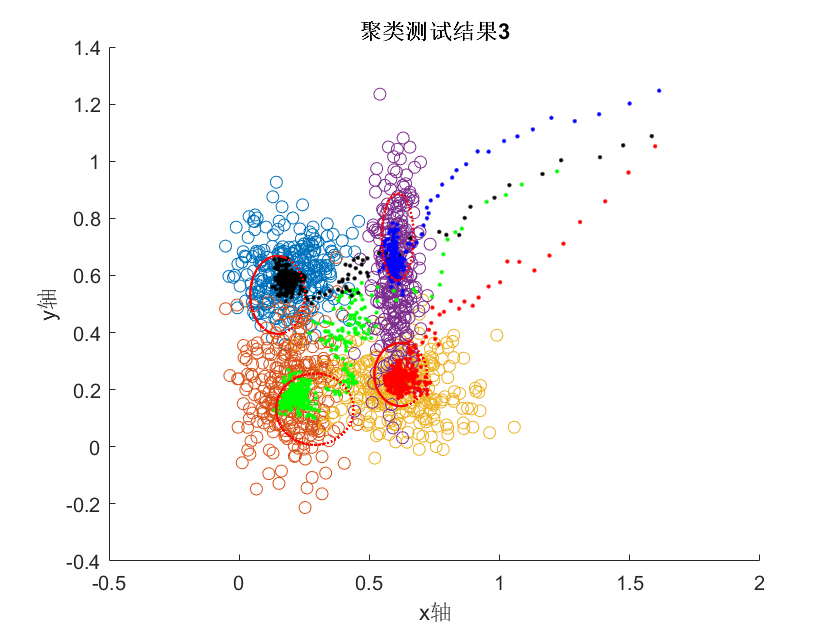
\includegraphics[width=0.7\textwidth]{ClusterTest3Result.png} % requires the graphicx package
   \caption{聚类测试3:起始点移动,结果图}
   \label{fig:clustest3re}
\end{figure}

可以发现其聚类效果仍然非常不错。聚类结果见表\ref{tab:clustest3},可见虽然中心存在一些偏差,但是已经准确地捕获到了聚类;如果输入更多数据将会改善其结果。数据方差值其实经历了一个先增大后减小的过程。
\begin{table}[htbp]
\centering
\begin{tabular}{c|c||c|c}
  \hline
  $\mu_{real}$   &  $\sigma_{real}$ &  $\mu$  &   $\sigma$\\
  \hline
  $(0.2,0.2)$    &  $(0.1,0.15)$   &  $(0.2905, 0.1316)$  & $(0.1482, 0.1250)$ \\
  $(0.2,0.6)$    &  $(0.1,0.1)$   &  $(0.1474, 0.5316)$  & $(0.1049, 0.1362)$ \\
  $(0.6,0.2)$    &  $(0.15,0.1)$   &  $(0.6200, 0.2530)$  & $(0.1011, 0.1103)$ \\
  $(0.6,0.6)$    &  $(0.05,0.2)$   &  $(0.6086, 0.7344)$  & $(0.0614, 0.1522)$ \\
  \hline
\end{tabular}
\caption{聚类测试3:聚类结果比较}
\label{tab:clustest3}
\end{table}

我们再将起始点范围更改为$(-5,0)$,其仍然可以很好的聚类,见图\ref{fig:clustest3-2re}。我们不再列出其参数结果。

\begin{figure}[htbp]
   \centering
   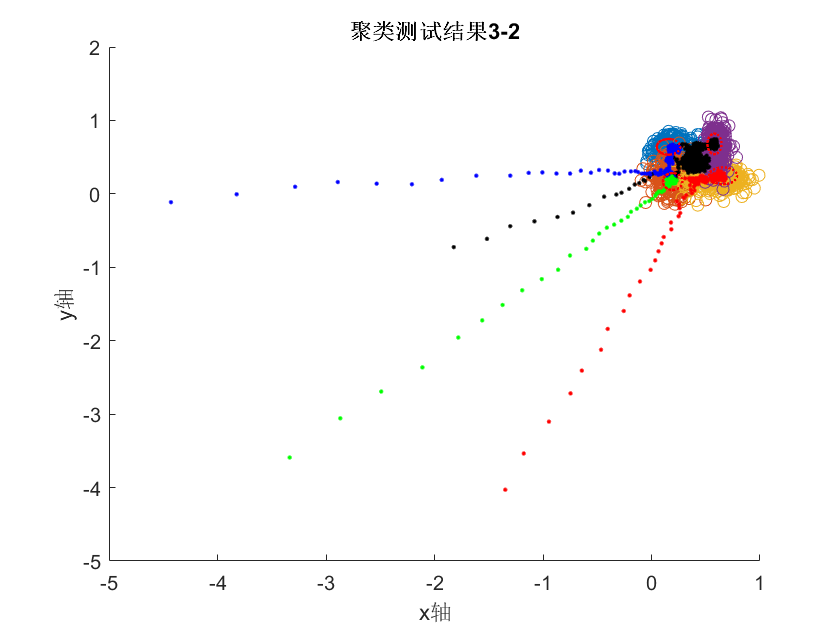
\includegraphics[width=0.7\textwidth]{ClusterTest32Result1.png} % requires the graphicx package
   \caption{聚类测试3-2:起始点大移动,结果图}
   \label{fig:clustest3-2re}
\end{figure}

\subsubsection{学习参数变化的影响}
学习参数$\alpha,\beta,\gamma$的选择是我们很关心的问题。学习参数在多大的范围内会对于聚类结果影响不敏感,这直接决定我们后期硬件设计是否要将其设置为变量的问题。

我们进行了多组$\alpha,\beta,\gamma$的测试,结果表明当$\alpha:0.05\sim 0.2,\;\beta:0.05\sim 0.2, \gamma: 0.95\sim 0.99$之间时,聚类效果较好,结果相对稳定。

图\ref{fig:clustest4re}展示$\alpha=0.2,\beta=0.2,\gamma=0.98$时的结果。

\begin{figure}[htbp]
   \centering
   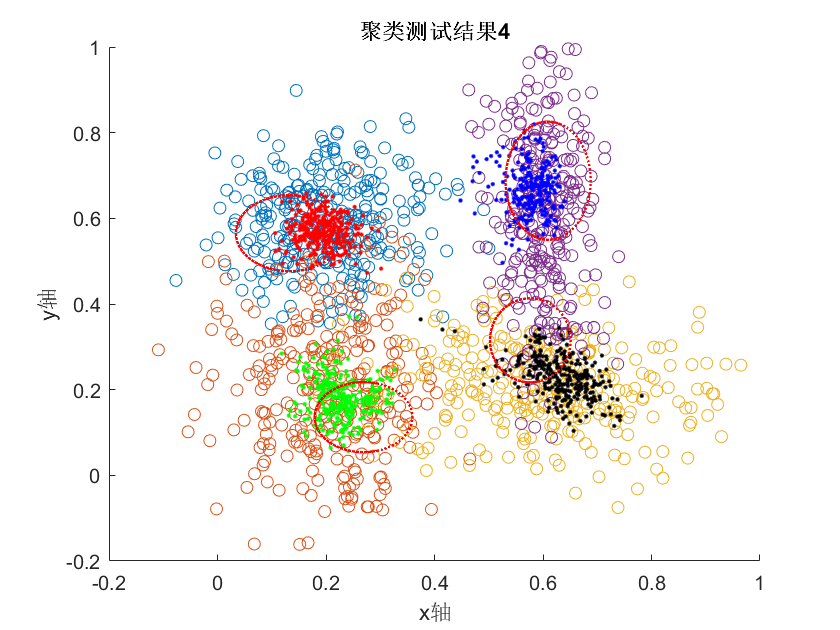
\includegraphics[width=0.7\textwidth]{ClusterTest4Result.png} % requires the graphicx package
   \caption{聚类测试4:学习参数调整,结果图}
   \label{fig:clustest4re}
\end{figure}

\begin{table}[htbp]
\centering
\begin{tabular}{c|c||c|c}
  \hline
  $\mu_{real}$   &  $\sigma_{real}$ &  $\mu$  &   $\sigma$\\
  \hline
  $(0.2,0.2)$    &  $(0.1,0.15)$   &  $(0.2692, 0.1358)$  & $(0.0901, 0.0818)$ \\
  $(0.2,0.6)$    &  $(0.1,0.1)$   &  $(0.1332, 0.5653)$  & $(0.0993, 0.0887)$ \\
  $(0.6,0.2)$    &  $(0.15,0.1)$   &  $(0.5766, 0.3151)$  & $(0.0743, 0.0981)$ \\
  $(0.6,0.6)$    &  $(0.05,0.2)$   &  $(0.6094, 0.6878)$  & $(0.0614, 0.1522)$ \\
  \hline
\end{tabular}
\caption{聚类测试4:聚类结果比较}
\label{tab:clustest4}
\end{table}

\subsubsection{聚类中心数目变化的影响}
聚类中心数目变化也是一个很重要的问题。 硬件设计时,很难考虑聚类数目随着数据灵活变化的问题;我们希望在聚类数目和真实的团簇数不一致的时候,聚类也能够有效地反映真实情况。

我们分别考虑聚类中心变多和变少两种情况。我们维持数据团簇数目$J_{real}=4$。

首先,我们令$J = 6$。聚类的结果如图\ref{fig:clustest5re}。

\begin{figure}[htbp]
   \centering
   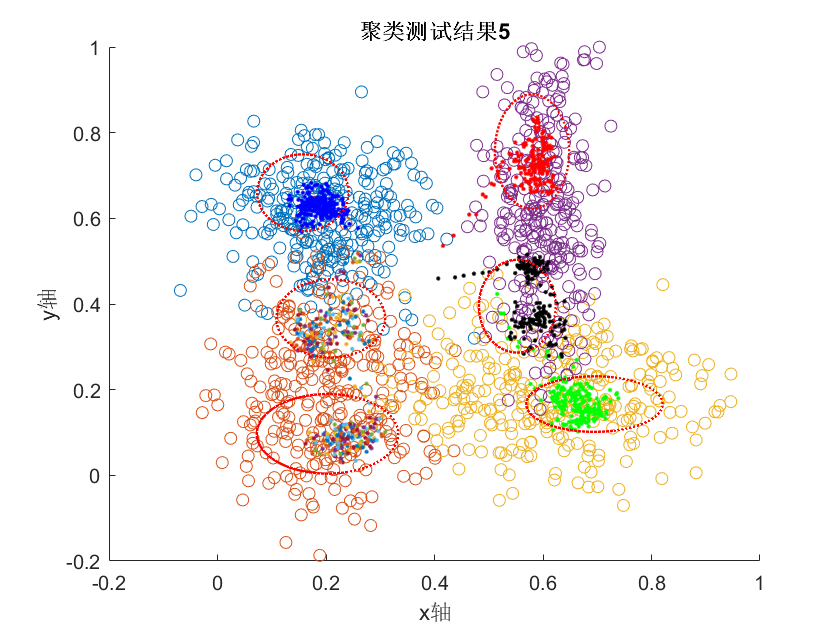
\includegraphics[width=0.7\textwidth]{ClusterTest5Result.png} % requires the graphicx package
   \caption{聚类测试5:聚类数目变多,结果图}
   \label{fig:clustest5re}
\end{figure}

可见聚类中心偏离了团簇的真实位置。然而,虽然聚类中心“过拟合”了团簇的真实情况,其对聚类的反映仍然基本正确。表列出了其聚类参数。

\begin{table}[htbp]
\centering
\begin{tabular}{c|c||c|c}
  \hline
  $\mu_{real}$   &  $\sigma_{real}$ &  $\mu$  &   $\sigma$\\
  \hline
  $(0.2,0.2)$    &  $(0.1,0.15)$   &  $(0.2088, 0.3663)$  & $(0.1002, 0.0913)$ \\
  $(0.2,0.6)$    &  $(0.1,0.1)$   &  $(0.1574, 0.6599)$  & $(0.0843, 0.0895)$ \\
  $(0.6,0.2)$    &  $(0.15,0.1)$   &  $(0.6849, 0.1664)$  & $(0.1256, 0.0649)$ \\
  $(0.6,0.6)$    &  $(0.05,0.2)$   &  $(0.5798, 0.7558)$  & $(0.0684, 0.1334)$ \\
  --    &  --   &  $(0.5527, 0.3949)$  & $(0.0708, 0.1083)$ \\
  --    &  --   &  $(0.2028, 0.0968)$  & $(0.1312, 0.0929)$ \\
  \hline
\end{tabular}
\caption{聚类测试5:聚类结果比较}
\label{tab:clustest5}
\end{table}

然后,我们减少聚类的个数,令$J = 2$。图\ref{fig:clustest5-2re}为两个聚类时的测试结果。可以看出聚类效果不是很理想,两个聚类中心不能找到任何一个特定的聚类中心,方差较大。
\begin{figure}[htbp]
   \centering
   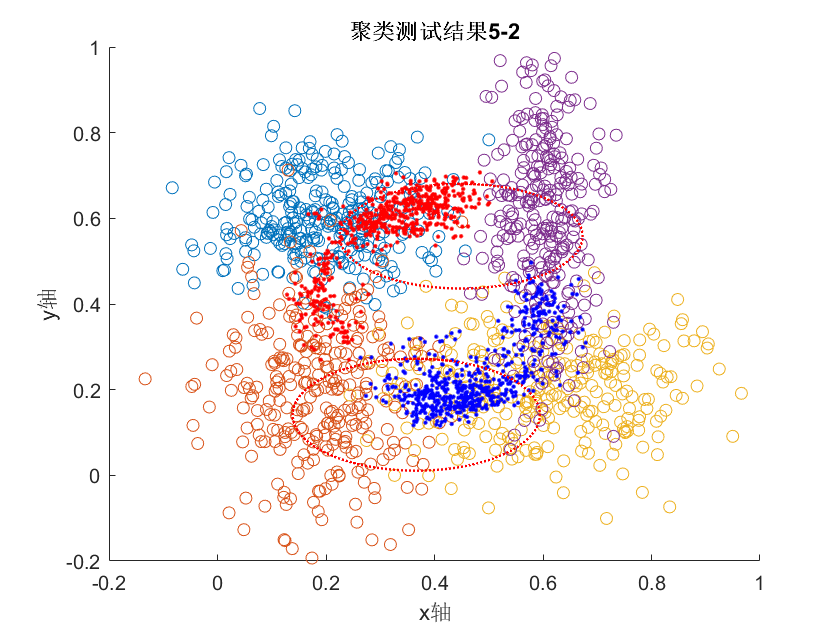
\includegraphics[width=0.7\textwidth]{ClusterTest52Result.png} % requires the graphicx package
   \caption{聚类测试5-2:聚类数目变少,结果图}
   \label{fig:clustest5-2re}
\end{figure}

聚类中心结果如表\ref{tab:clustest5-2}。

\begin{table}[htbp]
\centering
\begin{tabular}{c|c||c|c}
  \hline
  $\mu_{real}$   &  $\sigma_{real}$ &  $\mu$  &   $\sigma$\\
  \hline
  $(0.2,0.2)$    &  $(0.1,0.15)$   &  $(0.4491, 0.5583)$  & $(0.2239, 0.1222)$ \\
  $(0.2,0.6)$    &  $(0.1,0.1)$   &  $(0.3664, 0.1415)$  & $(0.2278, 0.1307)$ \\
  $(0.6,0.2)$    &  $(0.15,0.1)$   &  --  & -- \\
  $(0.6,0.6)$    &  $(0.05,0.2)$   &  --  & -- \\
  \hline
\end{tabular}
\caption{聚类测试5-2:聚类结果比较}
\label{tab:clustest5-2}
\end{table}

\subsubsection{聚类测试小结}
至此,我们总结出聚类的规律如下:
\begin{enumerate}
\item 起始位置对于聚类结果的影响很小;但是当数据点量较小时,将起始点初始化在数据范围内会使得其对聚类的捕捉更为迅速;
\item 在一定范围内(本实验为$\alpha:0.05\sim 0.2,\;\beta:0.05\sim 0.2, \gamma: 0.95\sim 0.99$),学习速率对聚类最终的结果影响不大,结果较为稳定;
\item 聚类数目比实际聚类数要多时,聚类的方差较小,对真实聚类情况能够有所反映;而聚类数目偏少时,不太能够有效地反映聚类的情况。后续测试应该将聚类数尽量设得多一些。
\end{enumerate}


\subsection{MNIST手写数字识别测试}
接下来我们进行了静态图像的识别测试。MNIST是一个常用的检测学习算法效果的手写数字集库。

在以下测试中,我们使用的DeSTIN结构为:
\begin{enumerate}
\item 底层输入层包含4*4个神经元,每个底层神经元接收底层图像4*4小单元的输入以及自身信度状态的反馈;底层神经元具有25个聚类;那么其输入维度为41维,输出维度为25维;底层的“视觉窗口”为16*16维;
\item 非底层神经元接收下属四个底层神经元的输入以及自身信度状态的反馈;同样地,其具有25个聚类;那么其输入维度为125维,输出维度为25维;
\item 整个DeSTIN结构分为3层:底层4*4,中间层2*2和顶层1*1,共21个神经元;
\item 在非底层神经元接收底层神经元信度状态输入的时候,底层神经元可以接收新图片的输入,构成流水线结构,如图\ref{fig:pipeline}。
\end{enumerate}

\begin{figure}[htbp]
   \centering
   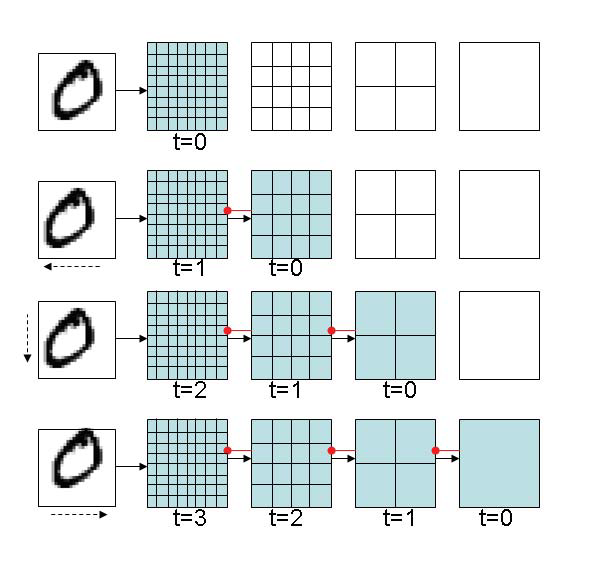
\includegraphics[width=0.7\textwidth]{ScanningPipeline.png} % requires the graphicx package
   \caption{DeSTIN结构与流水线}
   \label{fig:pipeline}
\end{figure}


\subsubsection{深度学习网络基本测试流程}
我们首先来介绍一下在使用DeSTIN(或者其他深度学习特征提取网络)进行数据测试的基本过程。首先,我们需要具有大量的无标签的数据,以及少量有标签的数据。我们将数据分为\uline{无标签训练集,有标签训练集,有标签测试集}三个部分。

那么,整个训练将分为三个步骤:
\begin{enumerate}
\item 通过大量无标签数据,训练DeSTIN网络,让其产生较好的聚类结果,如图\ref{fig:step1};
\item 关闭DeSTIN网络的训练,输入有标签的训练数据,训练后面的监督学习网络(本文中我们采用二层普通神经网络),如图\ref{fig:step2};
\item 关闭监督学习网络的训练,输入测试数据,测试其预测的结果,如图\ref{fig:step3};
\end{enumerate}

\begin{figure}[htbp]
   \centering
   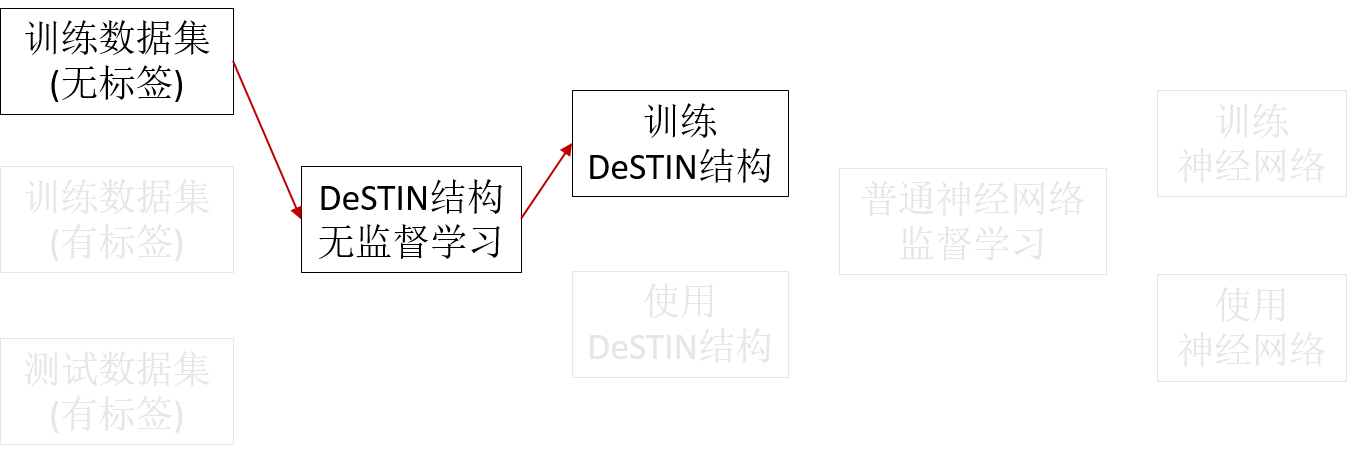
\includegraphics[width=0.7\textwidth]{DeSTINStep1.png} % requires the graphicx package
   \caption{测试过程1:无监督网训练}
   \label{fig:step1}
\end{figure}

\begin{figure}[htbp]
   \centering
   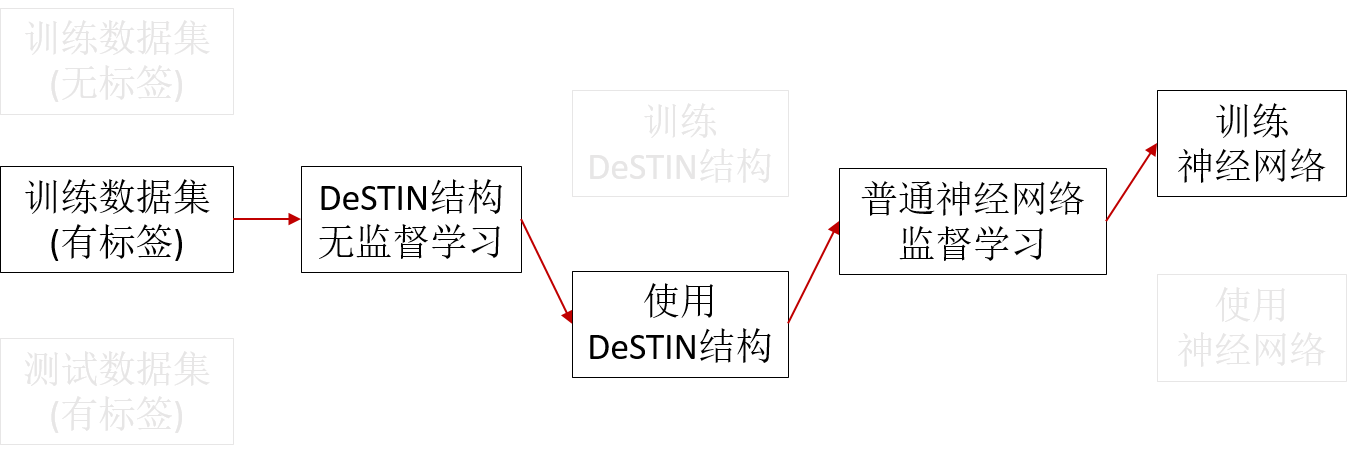
\includegraphics[width=0.7\textwidth]{DeSTINStep2.png} % requires the graphicx package
   \caption{测试过程2:有监督网训练}
   \label{fig:step2}
\end{figure}

\begin{figure}[htbp]
   \centering
   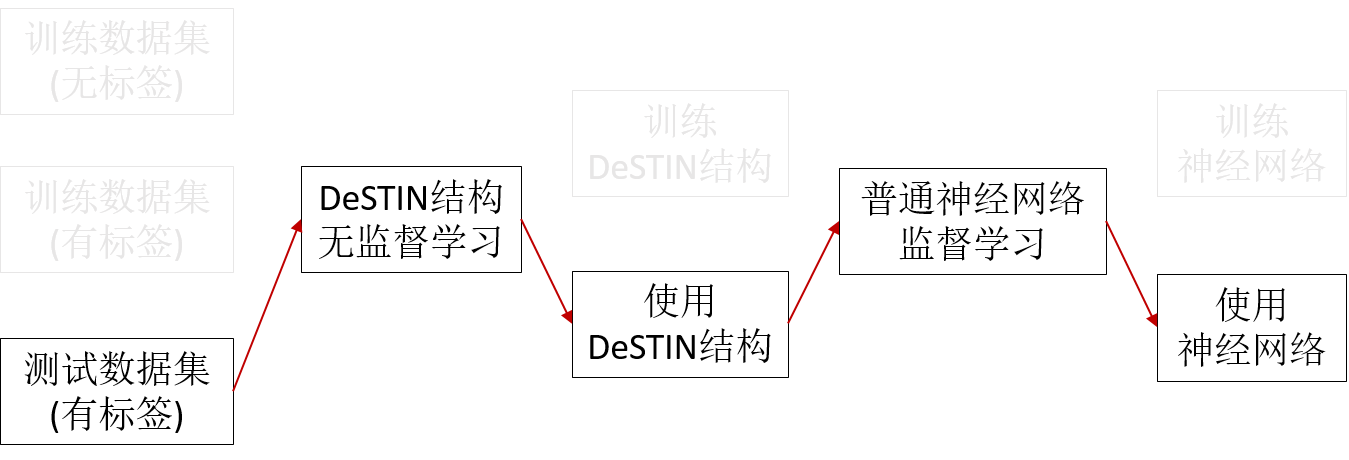
\includegraphics[width=0.7\textwidth]{DeSTINStep3.png} % requires the graphicx package
   \caption{测试过程3:预测过程}
   \label{fig:step3}
\end{figure}

\subsubsection{扫描方法的采用}
根据之前的分析,我们采用的DeSTIN算法在用来进行时间序列问题处理时比较合理,那么如何将其应用到静态图像识别上去呢?

在此我们借鉴了一个“视觉扫描”的理论:当人眼在看一件物品时,其注意中心是在进行不断的快速扫描的,这样可以防“视网膜”抖动,保持较高的分辨能力\cite{Deubel1996Postsaccadic}。

在这里我们模仿人眼的处理过程,让DeSTIN底层的“数据接收窗口”按照一个固定的顺序读取图像的每一个部分,这样就可以将静态的图像转换为动态的序列\cite{Karnowski2012Deep}。

此处我们首先采用简化的MNIST数据集,每一张手写数字图像为$20\times 20$像素点,我们架构的DeSTIN网络的“视觉窗口”为$16\times 16$那么我们采取图\ref{fig:scanning}的扫描方法,即让视觉窗口按照图示顺序平移,在进行到画圈处的时候,输出相应的信度状态。

\begin{figure}[htbp]
   \centering
   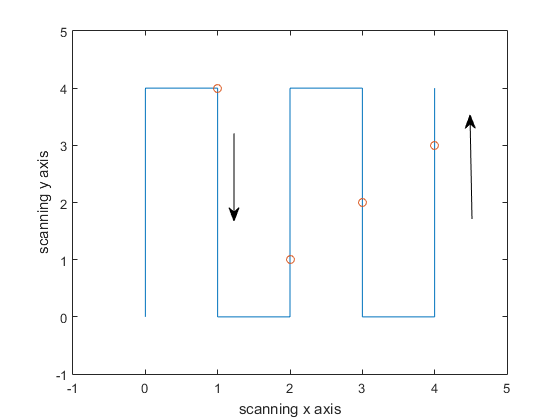
\includegraphics[width=0.7\textwidth]{ScanningImage.png} % requires the graphicx package
   \caption{“视觉扫描”识别的扫描顺序}
   \label{fig:scanning}
\end{figure}

我们将学习参数设置为$\alpha = 0.125, \beta = 0.125, \gamma = 0.9984$(第四章详细讲这样设置的原因)。测试集中,读入图片的前100张和相应的信度状态(前100维)的图像分别如\ref{fig:scanning}和图\ref{fig:belief}。

\begin{figure}[htbp]
   \centering
   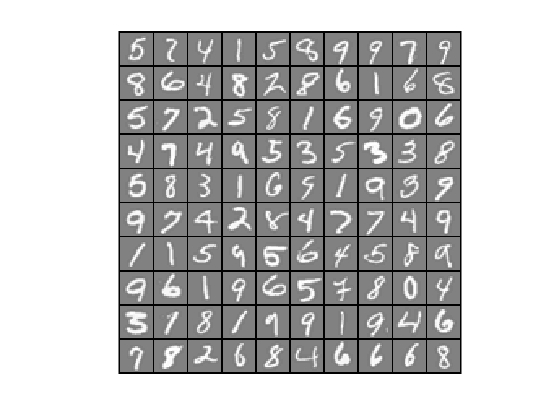
\includegraphics[width=0.7\textwidth]{MNISTSample.png} % requires the graphicx package
   \caption{MNIST测试的数字样本}
   \label{fig:scanning}
\end{figure}


\begin{figure}[htbp]
   \centering
   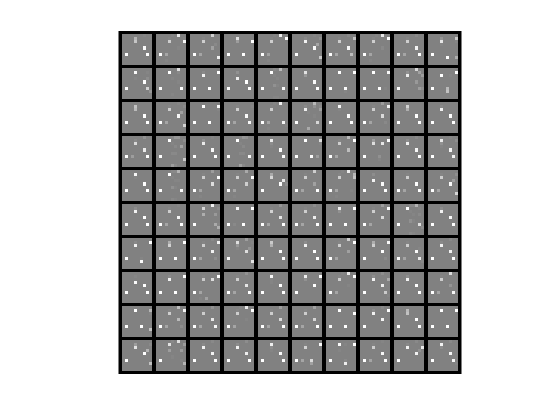
\includegraphics[width=0.7\textwidth]{MNISTResult.png} % requires the graphicx package
   \caption{MNIST测试DeSTIN网络输出的信度状态}
   \label{fig:belief}
\end{figure}

对于监督学习过程,我们采用普通的二层神经网络。 DeSTIN网络进行MNIST数据集测试训练的MATLAB代码将附在附录里面。我们得到了97.3\%的准确率。这说明我们的DeSTIN网络效果比较理想。

\subsubsection{学习参数变化测试}
我们再次在MNIST测试中测试结果对于学习参数的敏感情况。

首先,我们固定$\alpha = 0.125, \beta = 0.125$,改变$\gamma$,测试其准确率的变化如图\ref{fig:starverate}。可见当$\gamma:0.97\sim 0.99$时其准确度较高。

\begin{figure}[htbp]
   \centering
   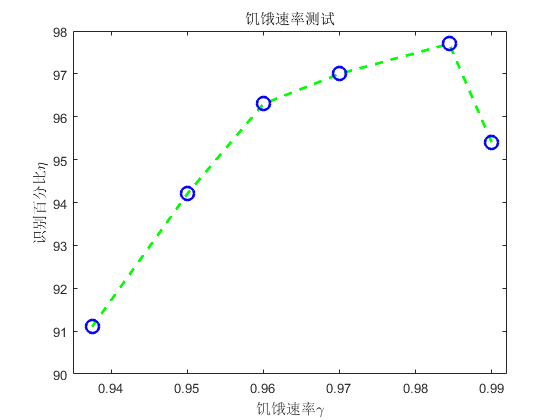
\includegraphics[width=0.7\textwidth]{StarveRate.png} % requires the graphicx package
   \caption{饥饿速率对准确度的影响}
   \label{fig:starverate}
\end{figure}

然后,我们固定$\gamma=0.9844$,在$0.05\sim 0.225$范围内,以$0.025$为步长遍历整个$\alpha,\beta$参数空间,最终获得的参数测试结果如图\ref{fig:learningrate}。

\begin{figure}[htbp]
   \centering
   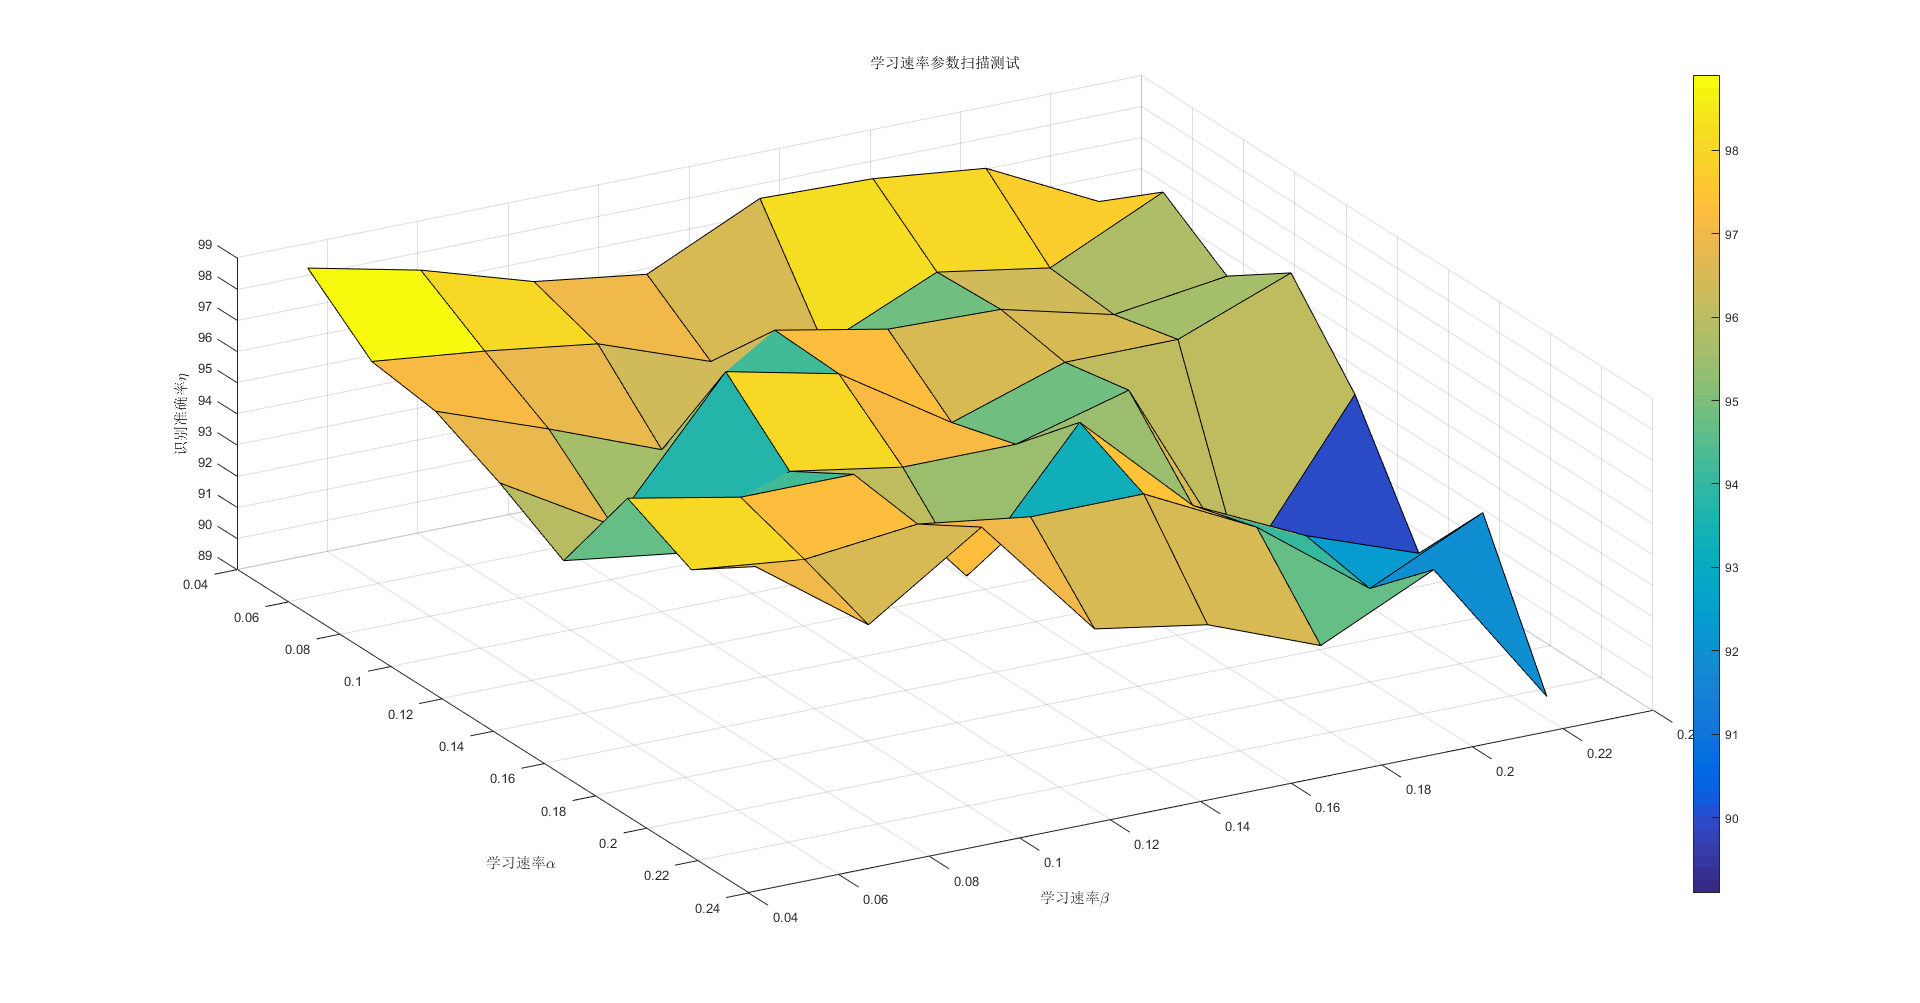
\includegraphics[width=\textwidth]{LearningRate.png} % requires the graphicx package
   \caption{学习速率对准确度的影响}
   \label{fig:learningrate}
\end{figure}

可见在$0.05\sim 0.2$的范围以内,学习速率对准确度影响很有限。考虑进方差的因素后,我们可以认为,准确度在此范围内对于学习速率不敏感。 这和前面聚类测试结果相吻合。

%\subsection{PEMS-SF数据集动态识别测试}
%动态识别仍在进行中,估计二稿整理出来

我们同样进行了标准的$28\times 28$大图像MNIST的测试,结果可以保持在$96\%$左右,同样相当理想。

\subsection{CIFAR物体识别测试与改进}
接下来我们想进行更加困难的测试:彩色物体识别。CIFAR是一个大型的彩色自然图像数据库\cite{CIFAR-10},其物体涵盖了大种类20种;小种类接近100种。其图像尺寸为$32\times 32\times 3$。图\ref{fig:cifar}展示了数据训练集的前100张图片。

\begin{figure}[htbp]
   \centering
   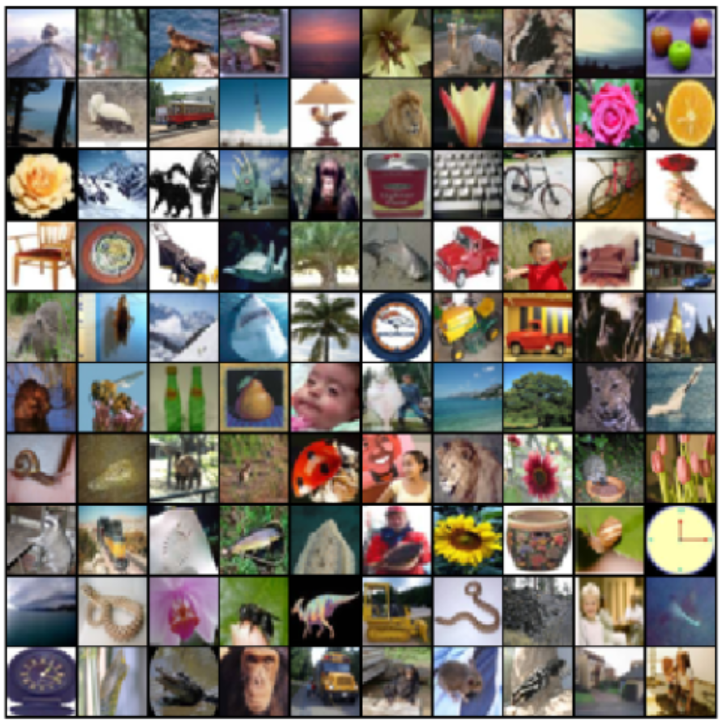
\includegraphics[width=0.7\textwidth]{cifar.png} % requires the graphicx package
   \caption{CIFAR数据集图例}
   \label{fig:cifar}
\end{figure}

我们按照MNIST的类似思路进行了CIFAR图像的训练(参考了Github上有关的Python代码\cite{pythonDeSTIN}),监督学习仍然使用了二层神经网络。

然而,我们最终只做出了最高$20.1\%$的准确度。

通过分析CIFAR测试失败的原因,我们发现的DeSTIN算法的固有缺陷:\textbf{对于位置的依赖关系严重}。当我们进行静态“扫描”识别的时候,很容易想象到,如果一个特征的位置发生了很大的变动:或者说,翻转、扭曲,这时候原来系统提取到的特征便不再吻合变化之后的物体。然而CIFAR数据集物体的位置特征比较混乱,这就导致识别的准确度大大降低。

我们在第二章讨论过有关\uline{卷积神经网络}的基本概念;卷积神经网络最早提出时,正是考虑到了我们刚刚讨论到的问题,认为\uline{一个图像内部的特征不会因为其线性变换而发生改变},因而提出了\uline{通过卷积核反映特征,卷积核对整个图像做卷积提取特征}的想法。

下一步我们对于DeSTIN算法将进行改进,在DeSTIN算法前面加上一层卷积、池化层,这样算法测试的结果应当能够得到较大改善。

%\bibliography{reference}